\chapter{Fabrication of field effect structures}\label{exfoliation}

The main goal of this thesis was to implement a fabrication pipeline for \tmdg monolayer samples, that yields narrow linewidth optical spectra and gate-tunability, enabling more accurate spectroscopic studies. This process builds on the work presented in \cite{funk_spectroscopy_2017}. Using the same mechanical exfoliation process in combination with standard micro lithography techniques and an advanced stamping procedure, this yields a fast and increasingly reliable process to build charge-tunable heterostructures of various \textsc{2d}-materials. 

\section{Mechanical exfoliation}
\begin{figure}
\centering
\begin{subfigure}{0.4\textwidth}
	\caption{}
	\begin{tikzpicture}
	\node[above right] (img) at (0,0) {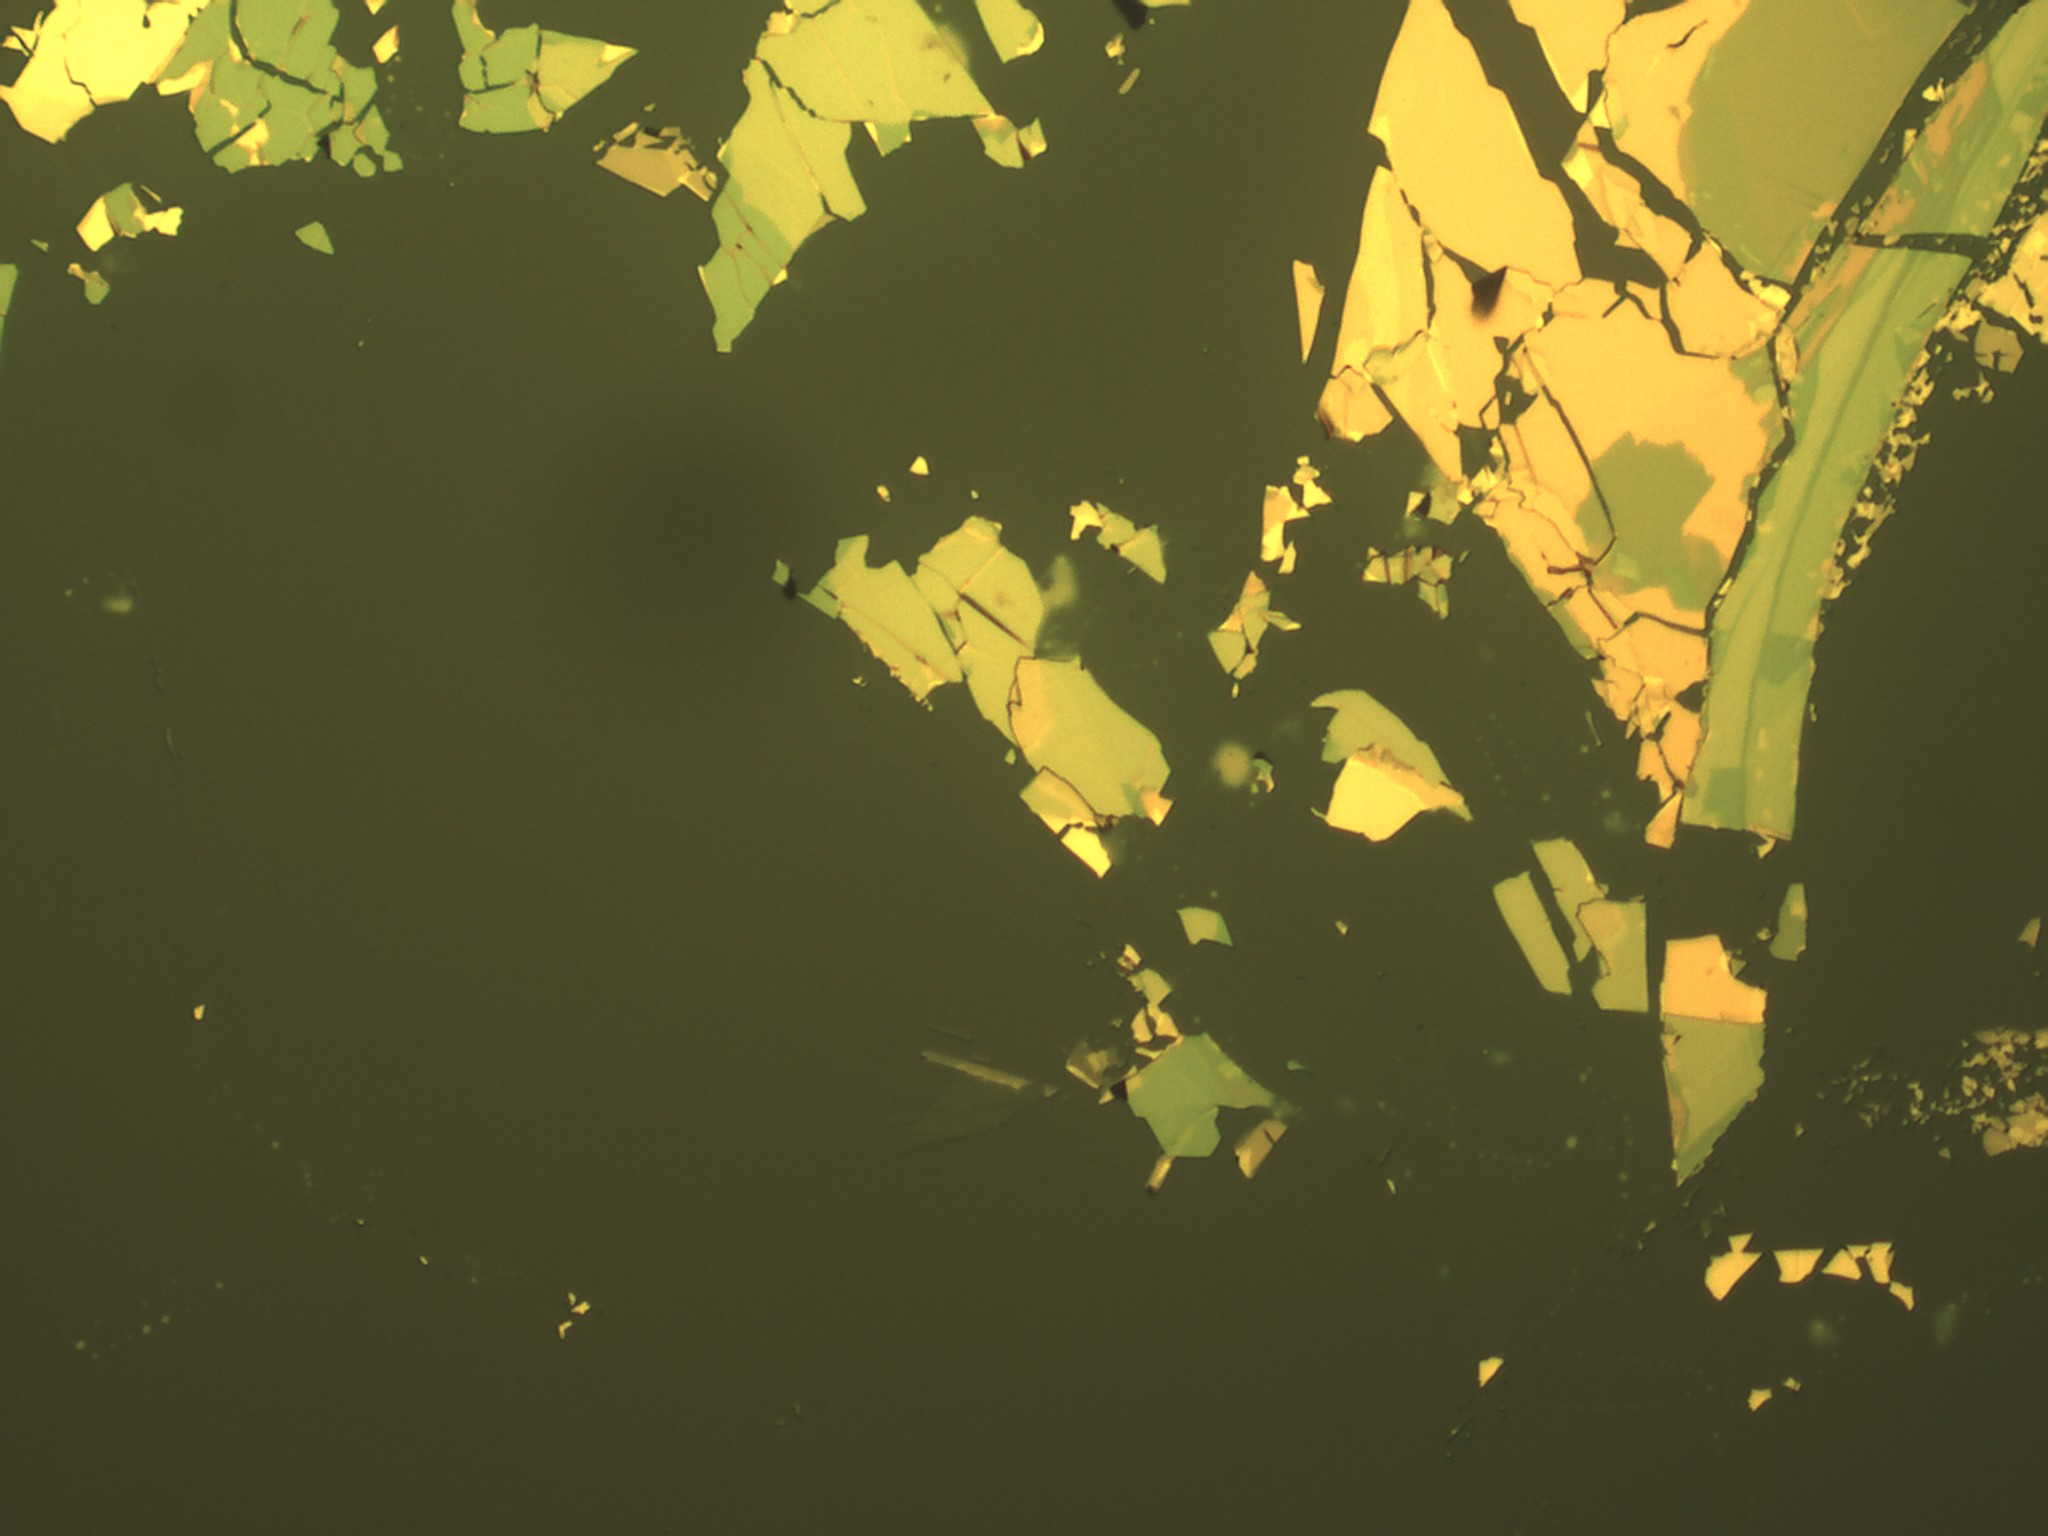
\includegraphics[width=\textwidth]{flakes.jpg}};
	\node at (84pt, 23pt) {{\large \textbf{ML/BL}}};
	\draw[red, dashed, thick] (83pt, 39pt) circle (9pt);
	\draw (20pt, 20pt) -- (60pt, 20pt);
	\node at (40pt, 12pt) {\textbf{100\mu m}};
	\end{tikzpicture}
\end{subfigure}
\begin{subfigure}{0.349\textwidth}
	\caption{}
	\begin{tikzpicture}
	\node[above right] (img) at (0,0) {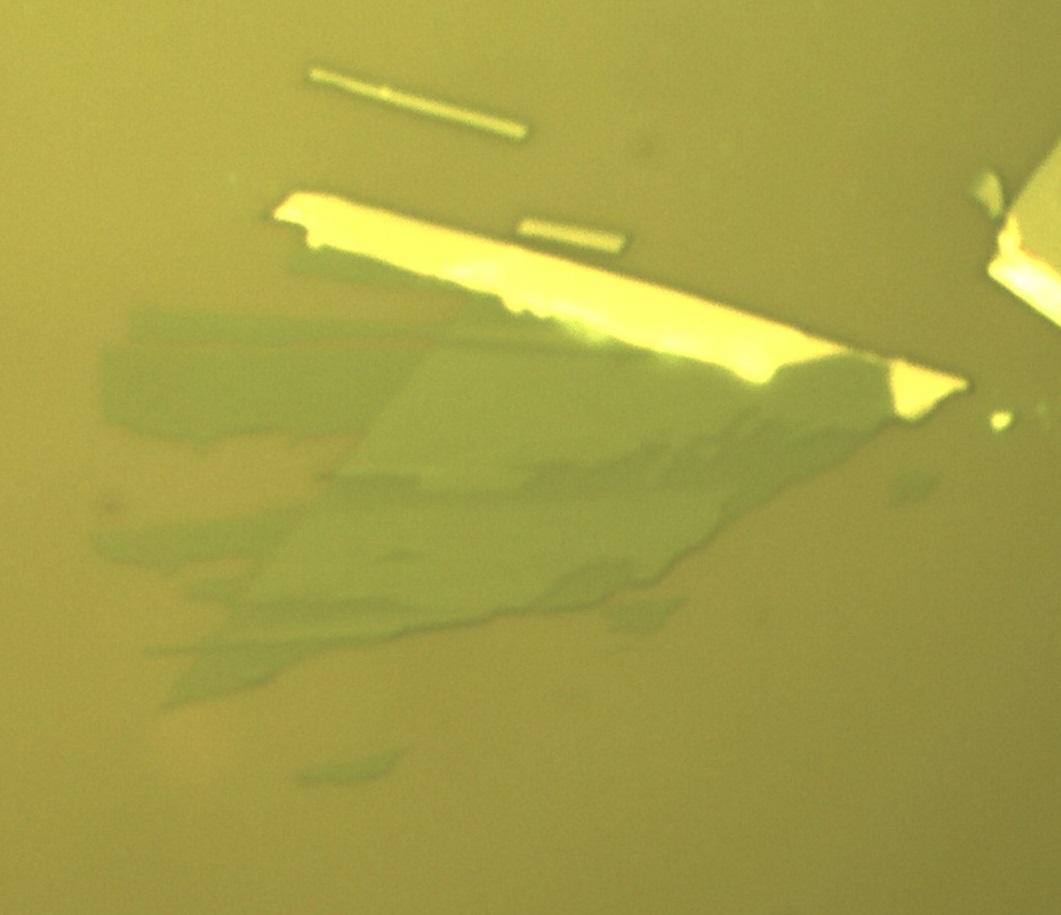
\includegraphics[width=\textwidth]{mono_on_sio2.jpg}};
	\node at (40pt, 80pt) {{\large \textbf{ML}}};
	\node at (65pt, 55pt) {{\large \textbf{BL}}};
	\draw (20pt, 20pt) -- (60pt, 20pt);
	\node at (39pt, 12pt) {\textbf{10\mu m}};
	\end{tikzpicture}
\end{subfigure}
\caption{\textbf{A} During the exfoliation process a lot of flakes of different size and thickness are scattered over the substrate. Interesting specimen have to be searched for by hand. \textbf{B} Flake consting of mono- and bilayer regions that can be identified by their optical contrast.}
	\label{flakes}
\end{figure}

Thin films of \tmds\!, like many natomaterials, can be fabricated using a top-down or bottom-up approach. Bottom-up these materials can be grown via chemical-vapor deposition (\textsc{cvd})\cite{chen_chemical_2016}. Because of its scalability it is the leading candidate for an industrial fabrication pipeline. However, the top-down approach of mechanical exfoliation has become the first choice for a lot of projects to build high quality model systems, that can be used to study physics in low dimensions\cite{geim_rise_2007}. The reason is the so far superior quality of few-layer flakes in terms of defects and contaminants as well as the synergy with dry transfer methods(See section \ref{hot_pickup}). 

The mechanical exfoliation process---often referred to as the ``scotch tape method''---is based on the fact, that the van-der-Waals forces between adjacent layers in \tmd's are much weaker, than the lateral covalent bonds---weak enough, that they can be easily broken apart by adhesive tape. The starting point is a solid crystal of \tmd-material, that can be produced either naturally or synthetically with high purity (supplied by hq-graphene). When a stripe of adhesive tape is brought in contact with it, a small amount can be peeled off. With a second stripe, that is put on the first one, the process is repeated multiple times. Each time, the fresh tape is peeled of its parent, the strong adhesion between tape and \tmdg ensures a clean interface. Three to four repetitions are an optimum to produce monolayers of a useful size. More repetitions further thin the material but heighten the risk of these thin films to break to smaller peaces, which complicates processing the flakes later on and build larger devices. 

To prepare monolayer flakes for the assembly of more complex devices, they first have to be transferred onto a suitible substrate. In this work, this substrate is silicon with a layer of thermal oxide that is between 50 and 90 nm thick. Before wafers of this material are brought in contact with the exfoliation tapes they are cleaned both in acetone and isopropanole before being exposed to oxygen plasma for 180 s. This ensures a clean surface and maximizes the material that sticks to the wafer(\cite{pizzocchero_hot_2016}). To release the tape the substrate is heated to 85°C for at least 2 minutes. After cooling down the tape can be peeled off and the wafer is inspected for monolayers. As seen in \ref{flakes}, this process yields a large number of flakes of different sizes and thicknesses on the substrate and it is common not to find a suitable monolayer sample on a typical \si-substrate (10 mm by 10 mm). 

\subsection{Layer number}

\begin{figure}
	\centering
	\begin{subfigure}{0.4\textwidth}
	\caption{}
	\begin{tikzpicture}
	\node[above right] (img) at (0,0) {\adjincludegraphics[trim={{.25\width} {.35\height} {.25\width} 0}, width=\textwidth, clip]{other_mono_bi.jpg}};
	\node at (80pt, 60pt) {{\large \textbf{ML}}};
	\node at (80pt, 150pt) {{\large \textbf{BL}}};
	\end{tikzpicture}
	\end{subfigure}
	\begin{subfigure}{0.4\textwidth}
	\caption{}
	\begin{tikzpicture}
	\node[above right] (img) at (0,0) {\adjincludegraphics[trim={ {.15\height} 0 {.1\height} 0}, width=.978\textwidth, clip, angle=90]{PL_imaging.png}};
	\node at (45pt, 45pt) {{\large \textbf{ML}}};
	\node at (100pt, 150pt) {\textcolor{white}{{\large \textbf{BL}}}};
	\end{tikzpicture}
	\end{subfigure}
	\caption{Comparison of mono- and bilayers of \wse\!. \textbf{A} The reflectance contrast of mono- and bilayers can be used to measure the layer number. The difference is however small enough to misidentify them under changing or inhomogenious lighting conditions. \textbf{B} The \pl-intensity of the monolayer is almost an order of magnitude higher than the bilayer and can therefore be identified very easily.}
	\label{pl-contrast}
\end{figure}

Under an optical microscope (Olympus® - \textsc{bh}2-\textsc{uma})monolayers can be identified using optical contrast and color as features to distinguish them from thicker films. It is possible to verify the layer number by this criteria alone using a camera and image analysis software\cite{funk_spectroscopy_2017}. However, this is much more reliable on transparent substrates, since the optical contrast is higher with an out-of-focus dark background. A reflective surface however enhances inhomogenities in the lighting conditions, making it harder to rely on absolute values of intensity. With our optical microscope and \si/\sio substrates, monolayer candidates where instead verified using photoluminescence (\textsc{pl}) imaging\cite{neumann_opto-valleytronic_2017}. In \tmds only monolayers show a direct band gap. Therefore even bilayers are much less efficient photonic emitters, showing almost an order of magnitude less \pl-intensity. The sample is excited with a laser with a wavelength above the direct exciton resonance and only the \textsc{pl} is collected on the chip of a \textsc{usb}-camera. A detailled description of the optical setup can be found in \ref{opticalsetup}. An sample measurement, comparing mono- and bilayer regions of \wse in a standard microscope image with \pl-imaging can be seen in figure \ref{pl-contrast}. 

Other methods to idetify monolayers inlcude both \pl and Raman spectroscopy\cite{zhao_lattice_2013,zhang_phonon_2015,tonndorf_photoluminescence_2013}. However, to fit in a fast assembly pipeline \textsc{pl}-imaging proved to be the best method to verify the layer number as well the overall quality of the sample.

\section{Hexagonal boron nitride}

For spectroscopic studies of \tmd's the right substrate plays a very crucial part. As discussed in section \ref{theory_exciton}, the ultra-thin geometry of \tmdg monolayers makes them very sensitive to the dielectric environment. To obtain a narrow linewidth of the spectral features both in reflection and \pl spectroscopy, a suitable substrate has to fulfill some important specifications. A minimal surface roughness---ideally be atomically flat---avoids local modulation of the band structure through strain. Also, the substrate has to be dielectrically calm to avoid local doping effects, that just like strain can introduce localized potentials, that broaden the linewidth. Both criteria rule out traditional substrates such as \si\ and \sio\!. In recent years hexagonal boron nitride (\hbn) has proven to be the superior choice to observe narrow linewidth spectra in \tmd's\cite{courtade_spectrally_2018}. \textsc{Hbn}, just like \tmds is a layered material, but belongs to the class of 2\textsc{d}-isolators, with a large, indirect band gap in the \textsc{uv}-range\cite{arnaud_huge_2006}. Thin, flat layers of \hbng can be mechanically exfoliated and achieve large, flat terraces. Few layers are sufficient to shield a \tmdg sample from the underlying substrate. To achieve even narrower lines, it can be ``sandwiched'' between two flakes of flat \hbng as was done with all samples contributing to this thesis. From the standpoint of nanofabrication \hbng has another important property. The van-der-Waals forces at \hbn-\tmdg interfaces are stronger than between \tmds and \sio\!. This is an important requirement for the hot pick-up assembly, discussed in section \ref{hot_pickup}.

\section{Electrode fabrication}

A gate-tunable \tmd-device can be understood as simple capacitor. A gate voltage is applied between the \tmd-flake and the doped \si\ substrate---separated by a 50 nm layer of thermal \sio\!.

\subsection{Top gate electrode}

\begin{figure}
\centering
\begin{subfigure}{0.4\textwidth}
	\caption{}
	\begin{tikzpicture}
	\node[above right] (img) at (0,0) {	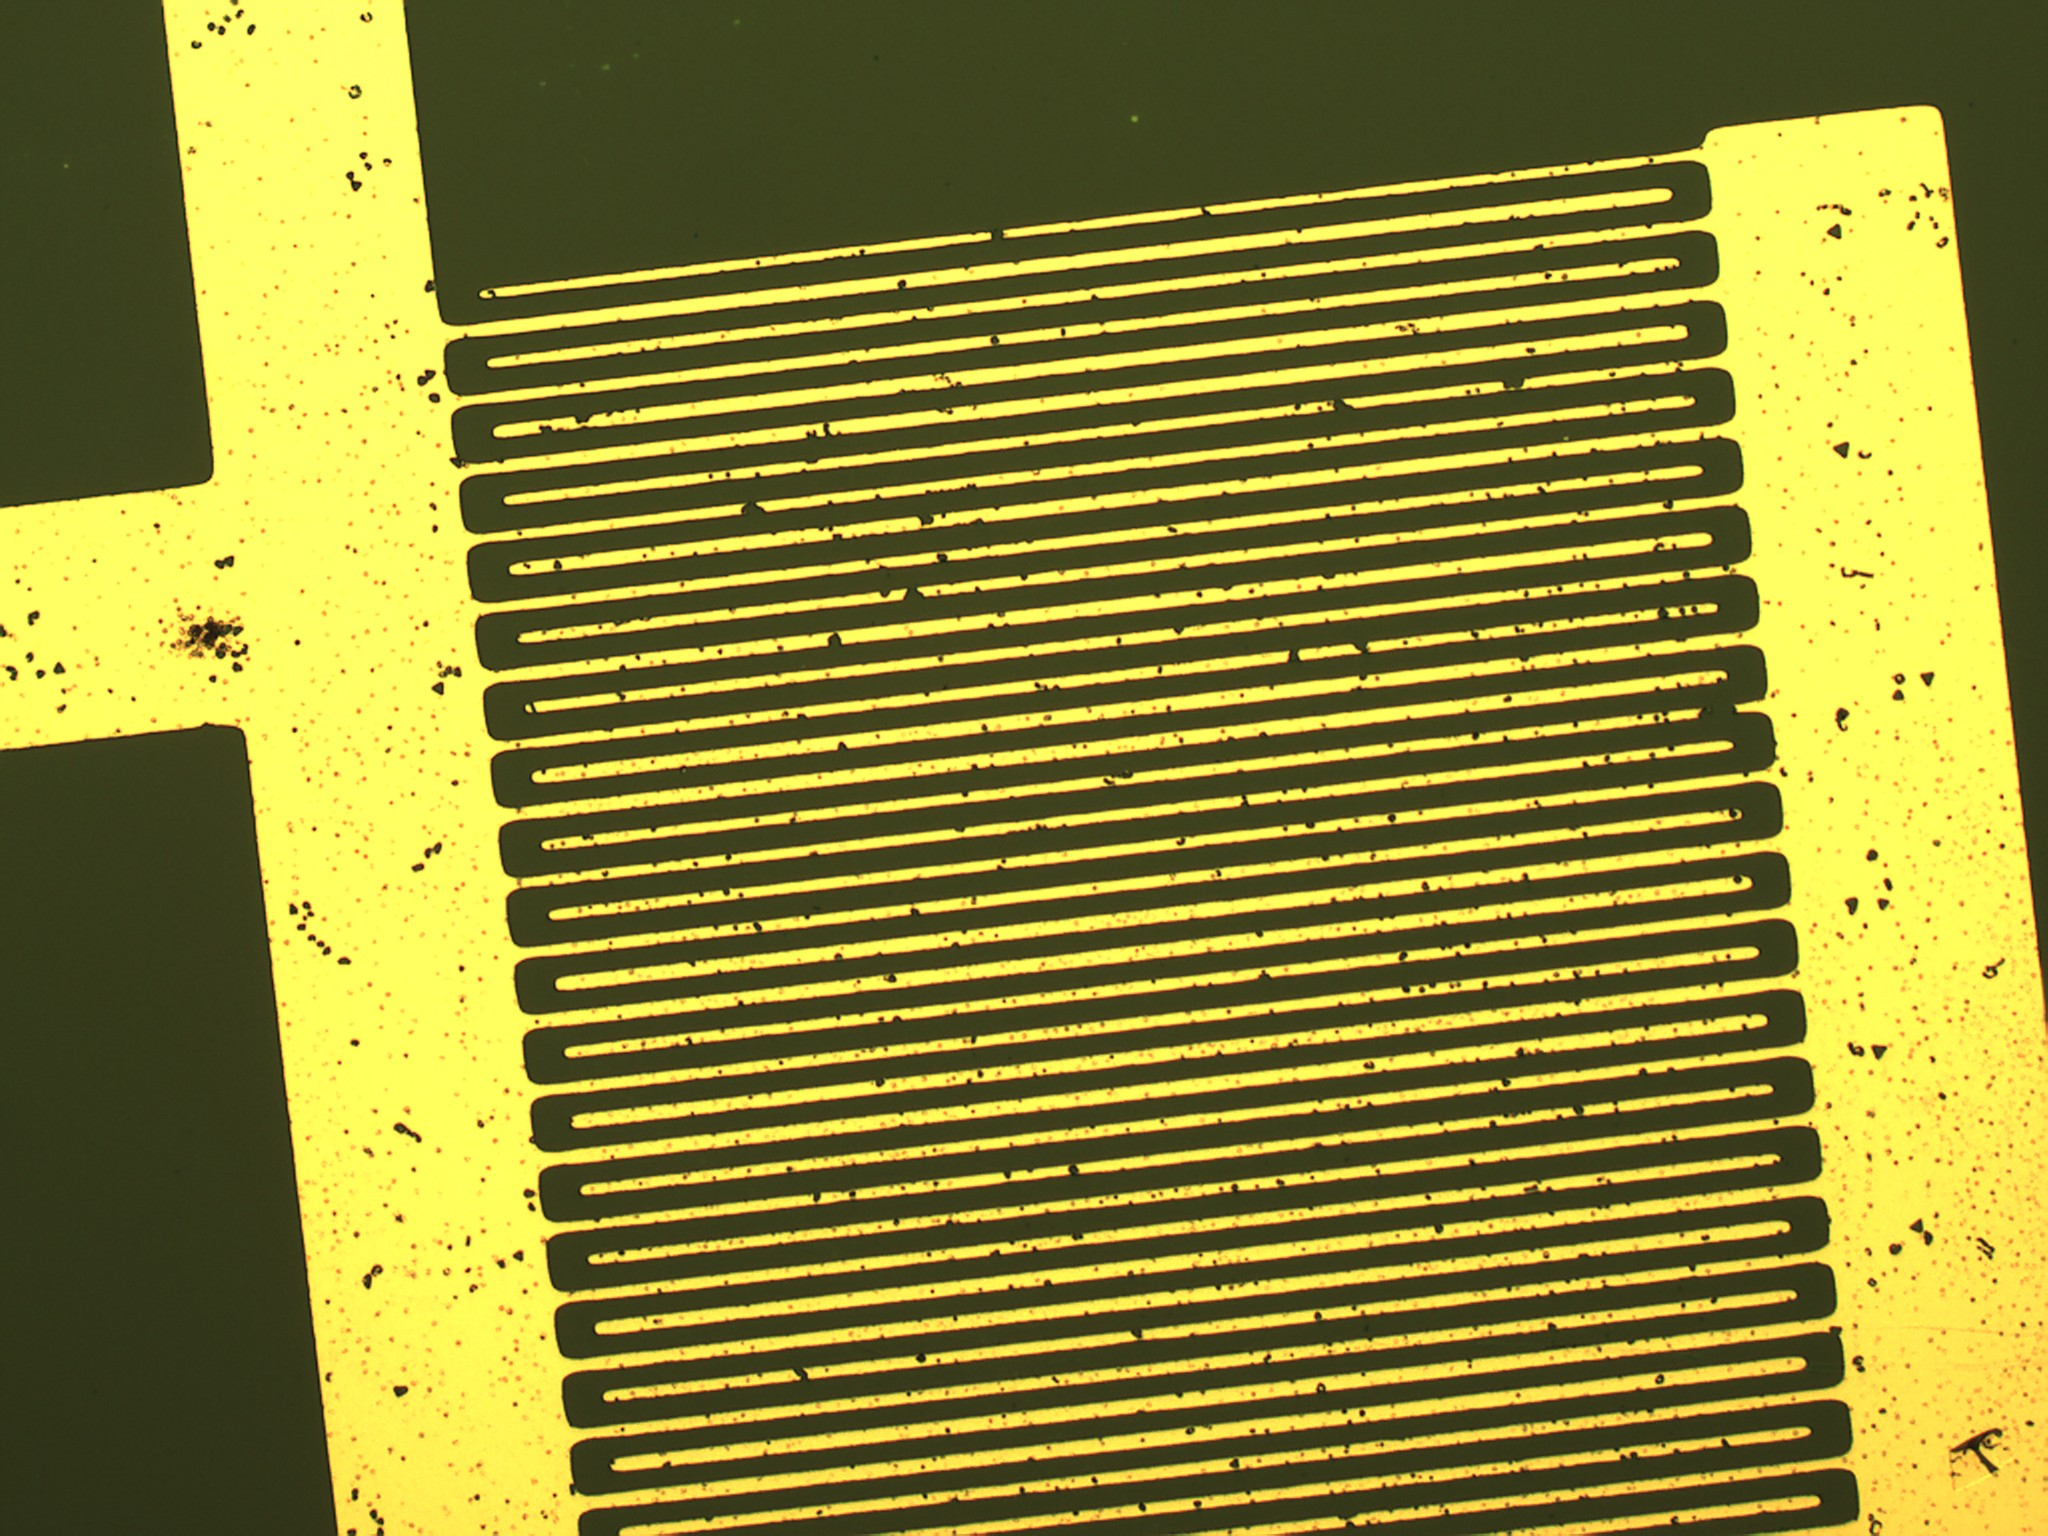
\includegraphics[width=\textwidth]{lithography.jpg}};
	\draw (20pt, 20pt) -- (60pt, 20pt);
	\node at (40pt, 12pt) {\textbf{200\mu m}};
	\end{tikzpicture}

\end{subfigure}
\begin{subfigure}{0.4\textwidth}
	\caption{}
	\begin{tikzpicture}
	\node[above right] (img) at (0,0) {	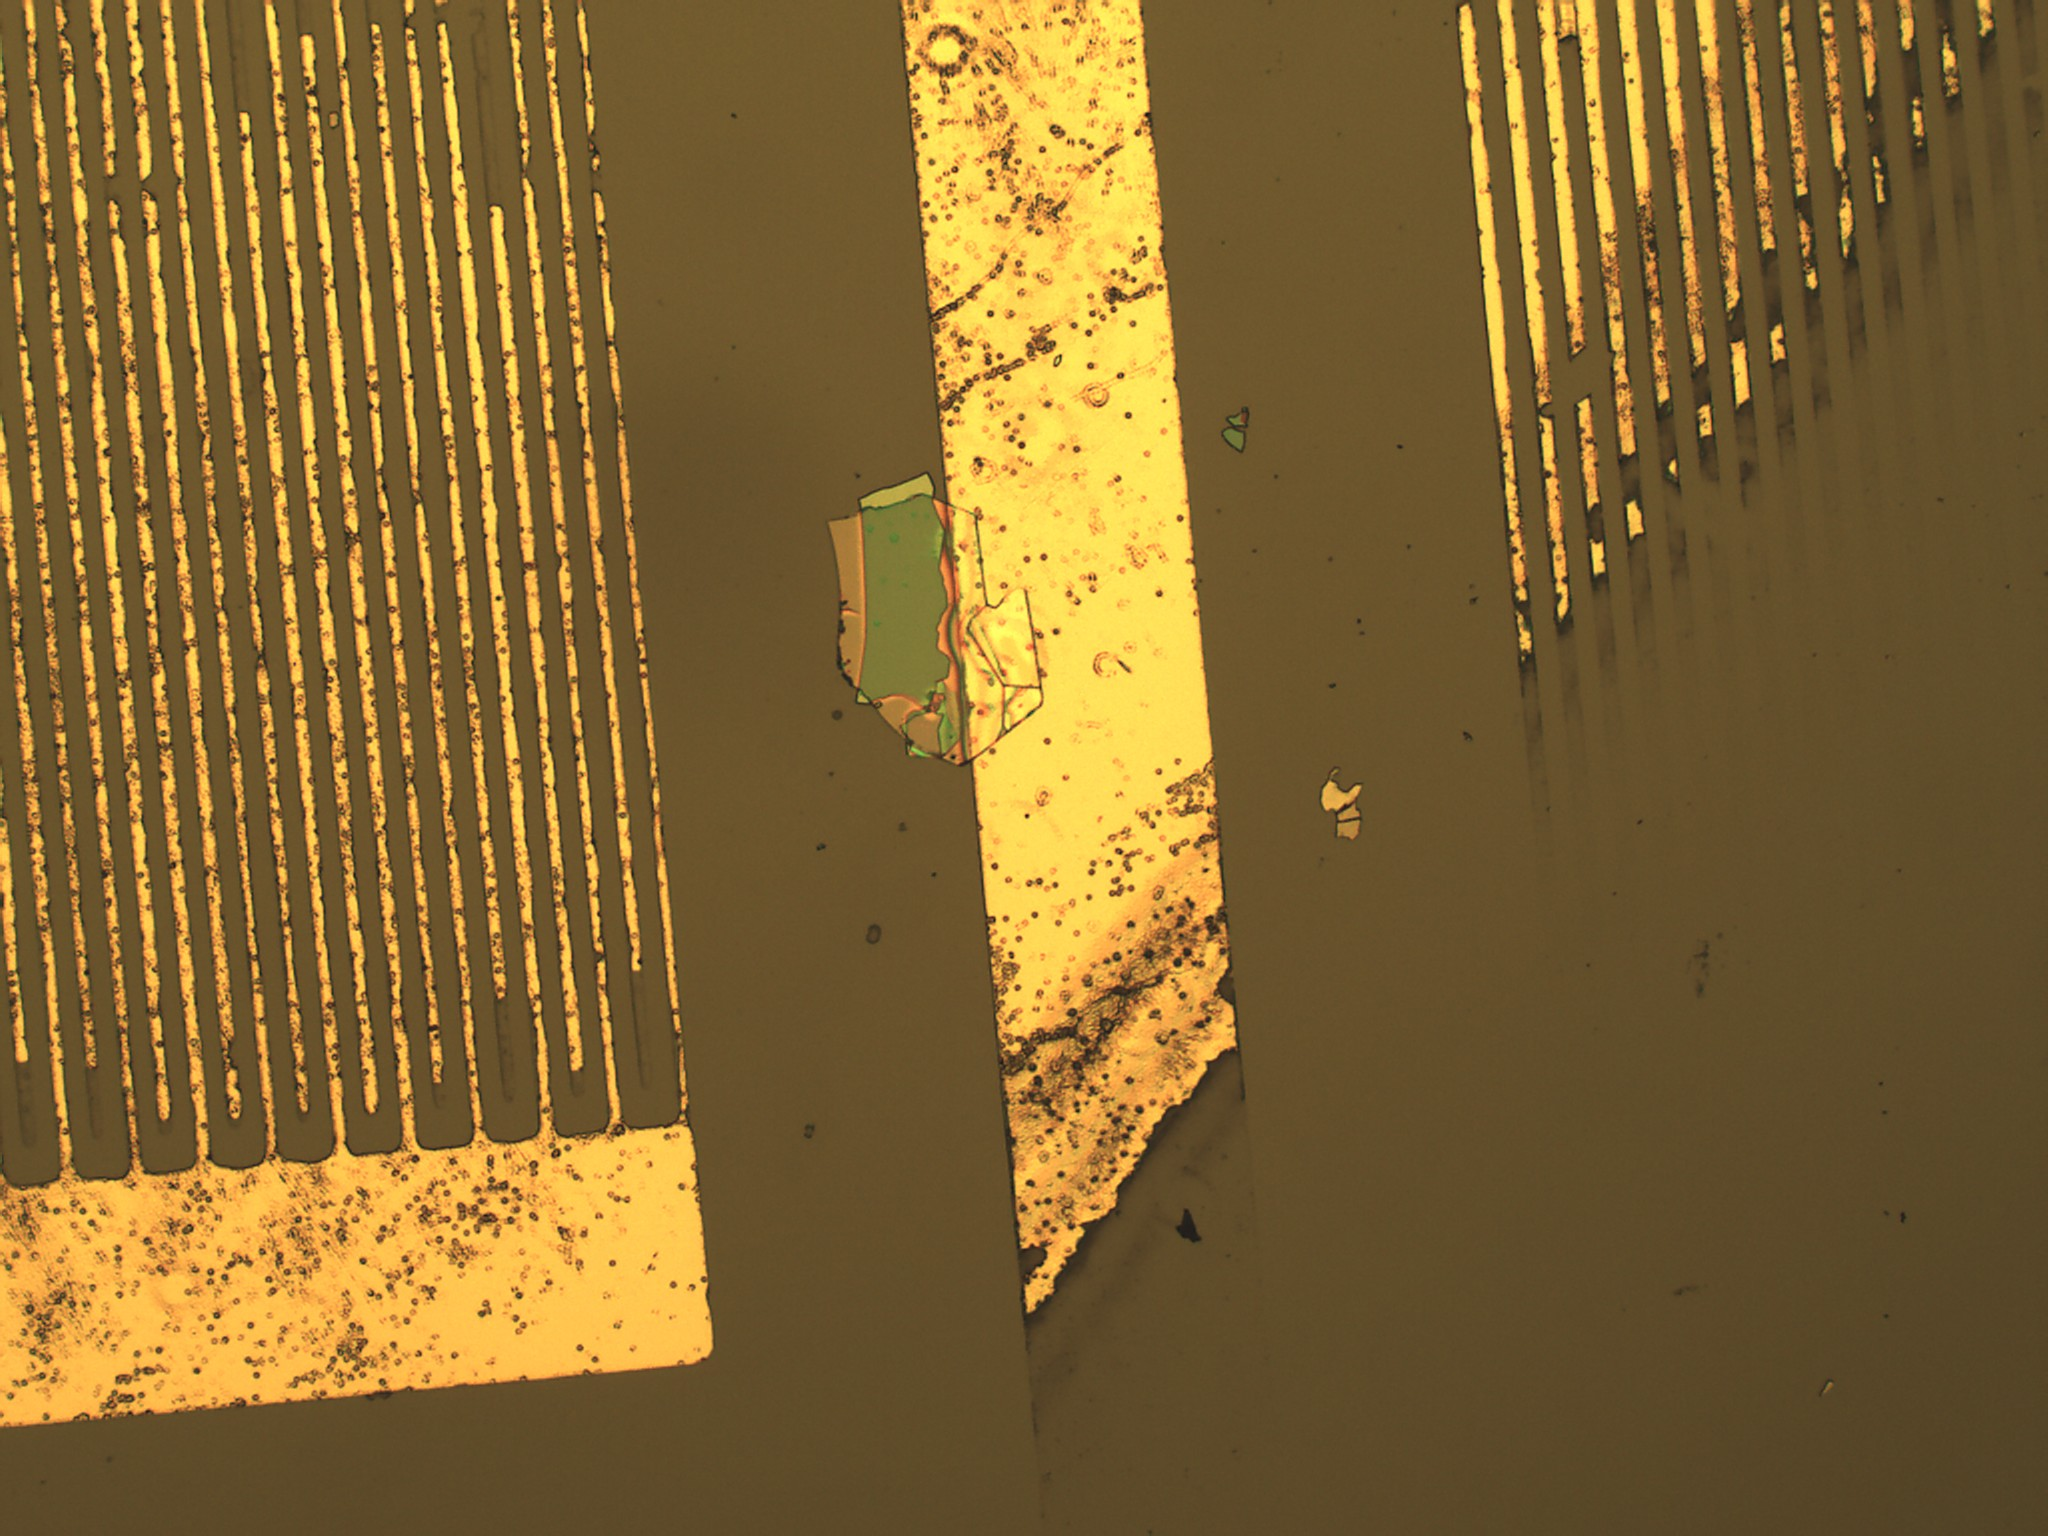
\includegraphics[width=\textwidth]{full_device.jpg}};
	\draw (120pt, 20pt) -- (160pt, 20pt);
	\node at (140pt, 12pt) {\textbf{200\mu m}};
	\end{tikzpicture}
\end{subfigure}
\caption{\textbf{A} Electrodes are written onto the substrate prior to the assembly of the \hbn-\tmdg heterostructure. A preused chromium mask of an interdigital structure is used for the gold pattern. \textbf{B} As long the heterostructure is dropped in contact with a thick line of the gold pattern, minor defects in the electrode structure do not affect the functionality of the device.}
	\label{pattern}
\end{figure}

To contact microscopic structures like \tmd-monolayers, electrodes have to be fabricated using micro-lithography. \textsc{Tmd} monolayers---either \textsc{cvd}-grown or exfoliated---are scattered on their substrates randomly. Therefore it is a common practice to fabricate electrodes directly on top of the sample via e-beam or laser lithography(Referenzen). Samples encapsulated in \hbng usually feature one or more additional films of graphene that provide an ohmic contact outside the heterostructure. Since only one contact is sufficient for charge-tunability, the process can be simplified greatly. Instead of writing electrodes after transfer, contacts are fabricated on the bare substrate. The encapsulated \hbn-\tmd-heterostructure can be contacted by dropping it on the edge of the gold structure. Most of the time, more \tmd-material than the monolayer is picked up during the transfer process. Because a \tmd-gold interface is conducting even at very low temperatures, these flakes provide suitable contacts, that do not have to be encapsulated in \hbn, therefore replacing additional graphene electrodes. Gold patterns are fabricated in contact lithography using a chromium mask that is deposited on glass. Because the stack can be dropped at any point on the substrate, the shape of the gold structure is unimportant, as long as it is large and connected. Therefore not even a new lithographic mask had to be fabricated. Instead a suitable mask was chosen from old pre-used structures. Even defects and deterioration of the masks only manifests aesthetically, rendering this process very robust and ideal for batch fabrication of gate-structures. The recipe starts with spin coating positive \textsc{az} 701 photoresist on a \si/\sio wafer. Using a maskaligner, the wafer is brought in contact with the chromium mask before exposing it to \textsc{uv}-light for 18 seconds. After that, the pattern is developed using \textsc{az} 826 \textsc{mif} developer, that washes out the exposed photoresist.

In the next step, the sample is coated in an X-ray evaporation system. First, a 1-5nm film of titanium is deposited on the substrate, that acts as a bonding agent. Subsequently a 50nm film of gold is deposited on top. After removing the sample from the vacuum chamber, the structures are finished in the so called ``lift-off''. The substrate is simply suspended in a solvent like acetone, that dissolves residual photoresist, only leaving gold, deposited in the developed. To speed up the lift-off process, the sample can be placed in an ultrasonic cleaner at a low power. The resulting structure can be seen in figure \ref{pattern}. 

\subsection{Back gate electrodes}

\begin{figure}
	\centering
	\resizebox{!}{150pt}{%
	\begin{tikzpicture}[scale=0.62, every node/.append style={transform shape},
        interface/.style={
        % The border decoration is a path replacing decorator. 
        % For the interface style we want to draw the original path.
        % The postaction option is therefore used to ensure that the
        % border decoration is drawn *after* the original path.
        postaction={draw,decorate,decoration={border,angle=-45,
                    amplitude=0.3cm,segment length=2mm}}},
        ]
	\begin{circuitikz}[american voltages]
		\draw (0,0) to[short] (0,0);
		\draw 
		(0,4) to[V, v=$20$V to $30$V] (0,0)
		(0,4) to[R, l=$3$k$\Omega$] (4,4)
		(0,0) to[short, *-] (4,0)
		(0,0) node[ground]{}
		(4,4) to[C, l=$1000$\mu F, *-*] (4,0)
		(4,4) to[short] (7,4)
		(7,4) to[short] (7,3)
		(7,3) to[short] (7.7,2.3)
		(7.7,2.3) node[inputarrow, rotate=315] {}
		(4,0) to[short] (7,0)
		(7,0) to[short] (7,1)
		(7,1) to[short] (7.7,1.7)
		(7.7,1.7) node[inputarrow, rotate=45] {}
		;
		\draw[line width=.5pt,interface] (8.1,0.7)--(8.1,3.2);
		\node at (8.2,3.6) {Substrate};
		\node at (6.8,2.05) {Gold wires};
	\end{circuitikz}
		
	\end{tikzpicture}
	}
	\caption{Circuit diagram for back gate fabrication: A capacitor is charged at 20V to 30V. Two boron-doped gold wires are moved very colesly to the silicon substrates. Once the distance between the wires and the substrate is low enough, an electric arc forms, discharging the capacitor through the substrate. Heat from the high current melts the tip of the gold wire locally doping the silicon and creating a gradient semiconductor/metal-interface.}\label{arc}
\end{figure}

Silcon is a semiconductor. A simple contact with a metal wire therefore results in a Schottky barrier at low temperatures. To create an ohmic contact to the backgate, the semiconcutor/metal interface is ``smeared out'' by diffusing boron doped gold into the substrate (see figure \ref{arc}). This is achieved by applying a high voltage between two gold wires and bringing them close to the substrate. Because the \si-substrate has a higher conductivity than the ambient air, an arc discharge between the tips of the wires will preferably find its way through the substrate. When the arc forms the tips of the gold wire evaporate and penetrate the \si-substrate. This creates a gradual metal-semiconductor interface and avoids a Schottky barrier, leaving a small gold droplet on the surface that can be contacted to a thin wire using conducting paste.

This process can be very violent. Gold droplets can splash over a large distance and evaporated gold can not only diffuse into the backgate but can also contaminate the \sio surface, lowering the breakdown voltage significantly. Therefore this step in the fabrication process should be taken before assembling the \tmd-\hbng heterostructure. This way, the substrate can be replaced in case of failure.

\section{Hot pick-up and transfer}\label{hot_pickup}

\begin{figure}
	\centering
	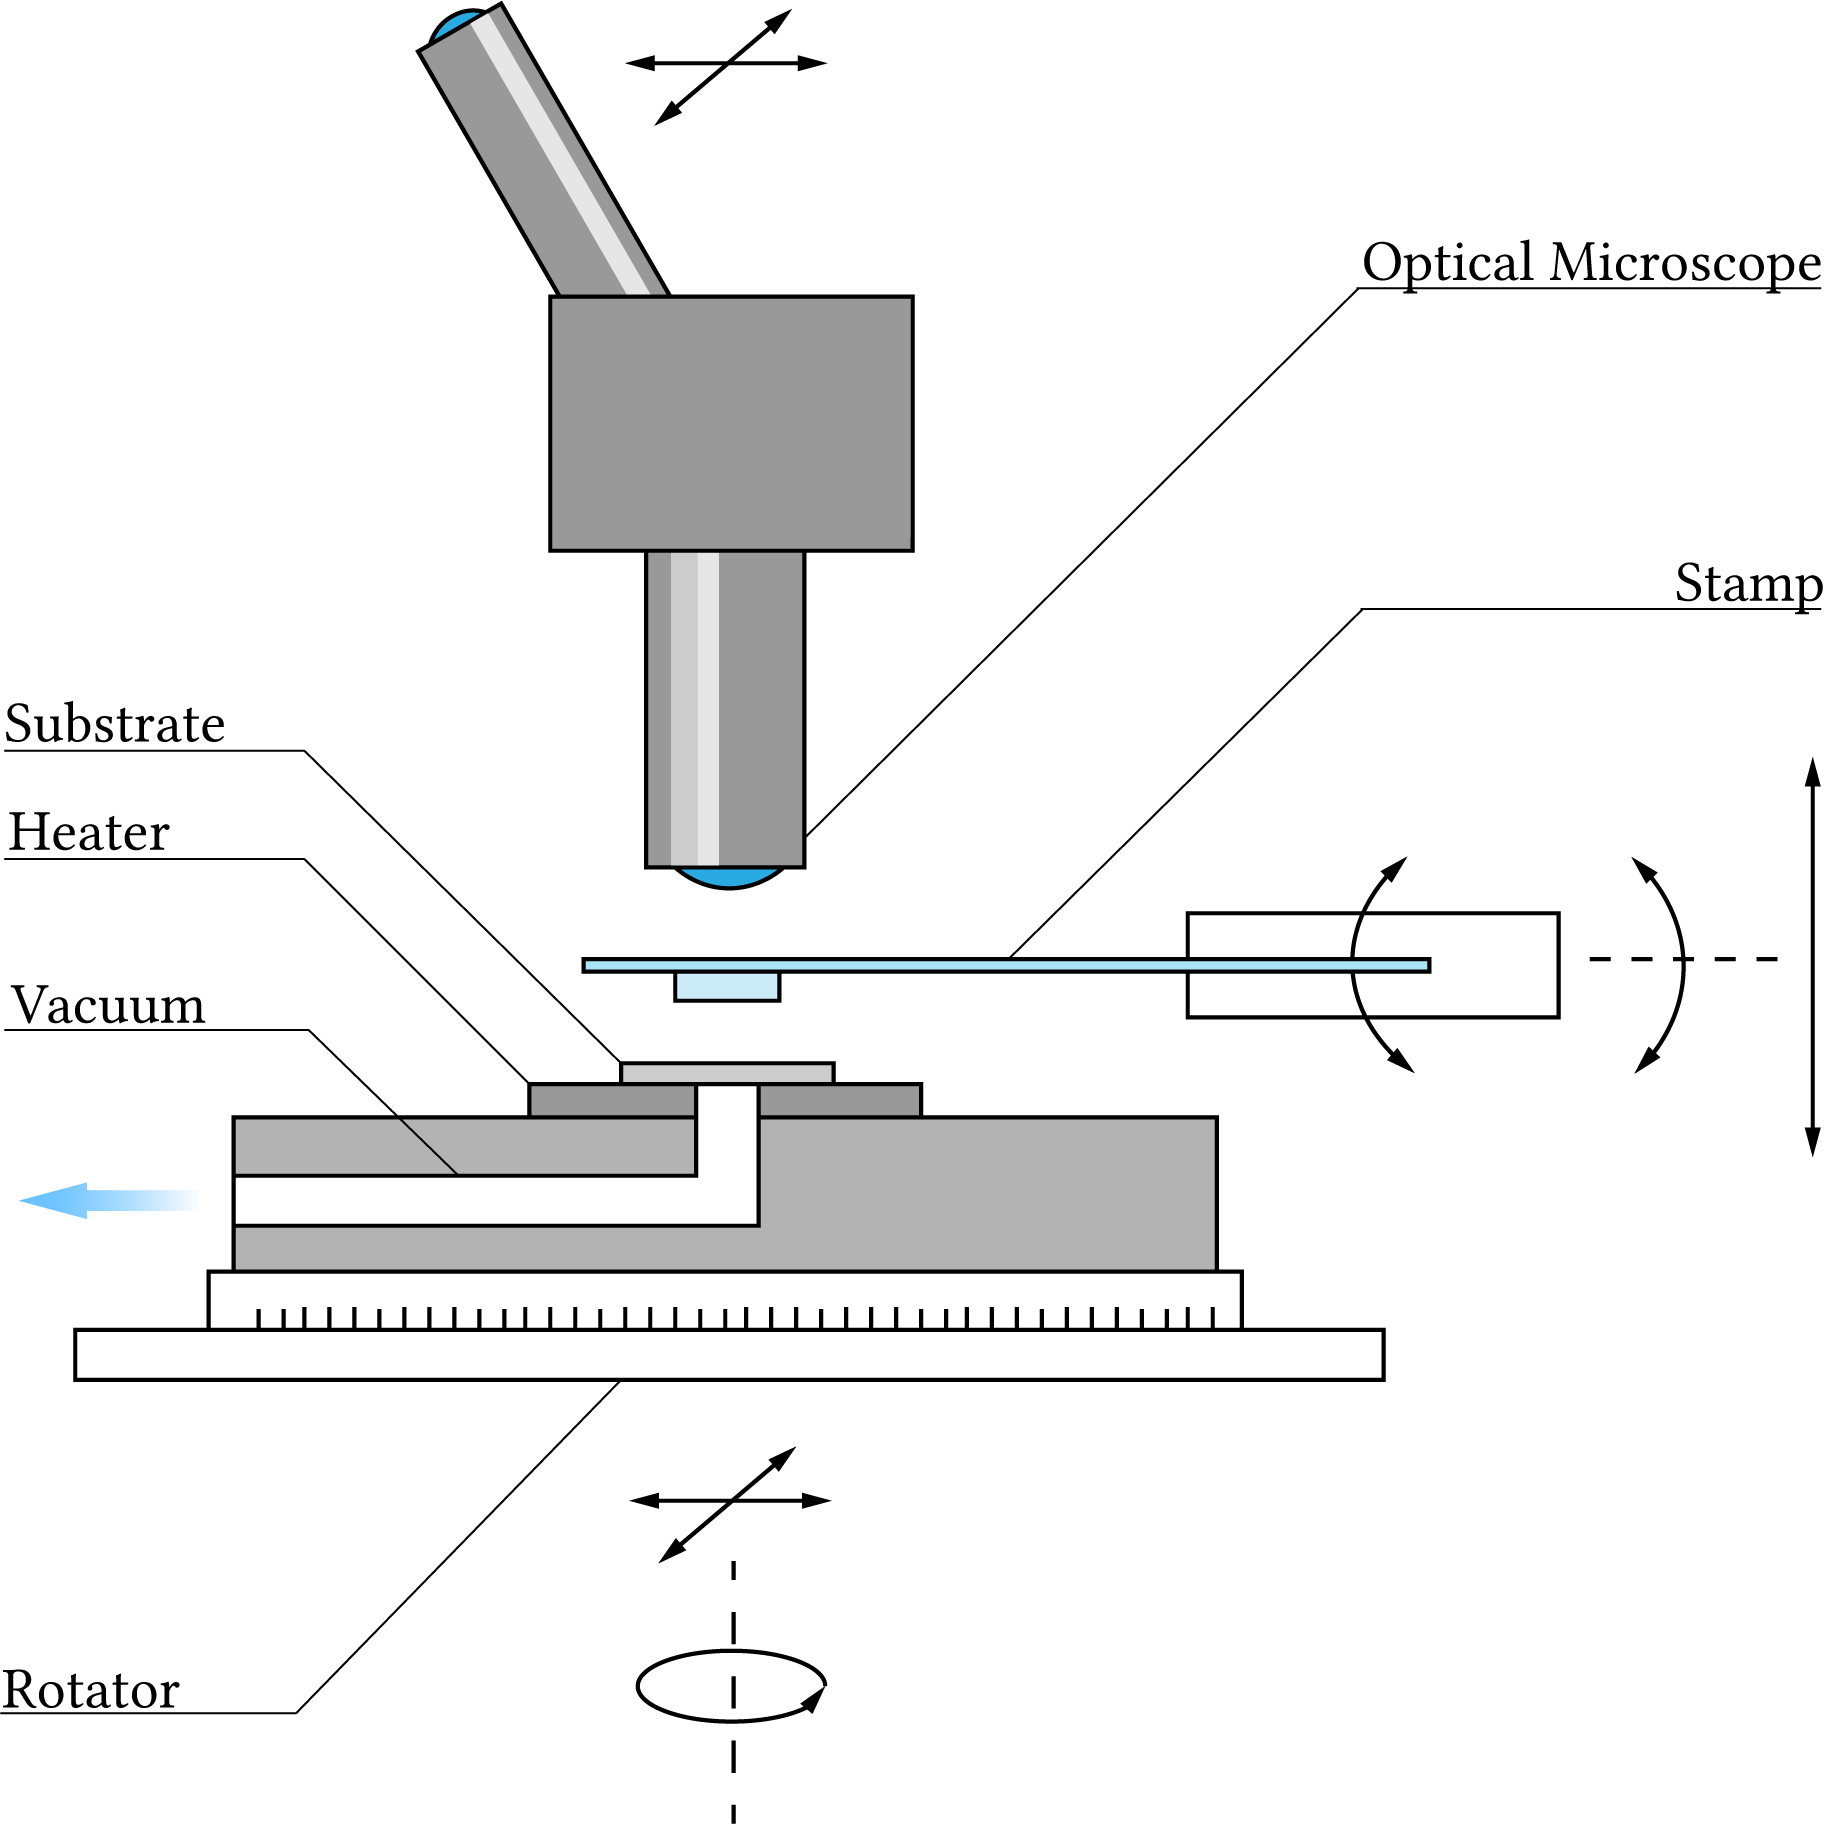
\includegraphics[width=0.7\textwidth]{Stempelaufbau.png}

	\caption{Setup for hot pick-up and stamping. The substrate is placed on a small, round \textbf{ceramic heater} with a 3mm whole in the center(Referenz Thorlabs), that is \textsc{pid}-controlled and can reach temperatures up to 200°C. It is mounted airtight onto the massive sample holder, that is connected to a \textbf{vacuum pump} to hold the \textbf{substrate} in place. It is \textbf{fully rotatable} and can be moved in plane. The \textsc{pdms/ppc} \textbf{stamp} is monted to a z-translator and can be tilted with respecto to both in-plane axes. The \textbf{optical microscope} can also be moved in-plane.}
	\label{stamping-setup}
\end{figure}


\begin{figure}[t]
\centering
\begin{subfigure}{0.49\textwidth}
 	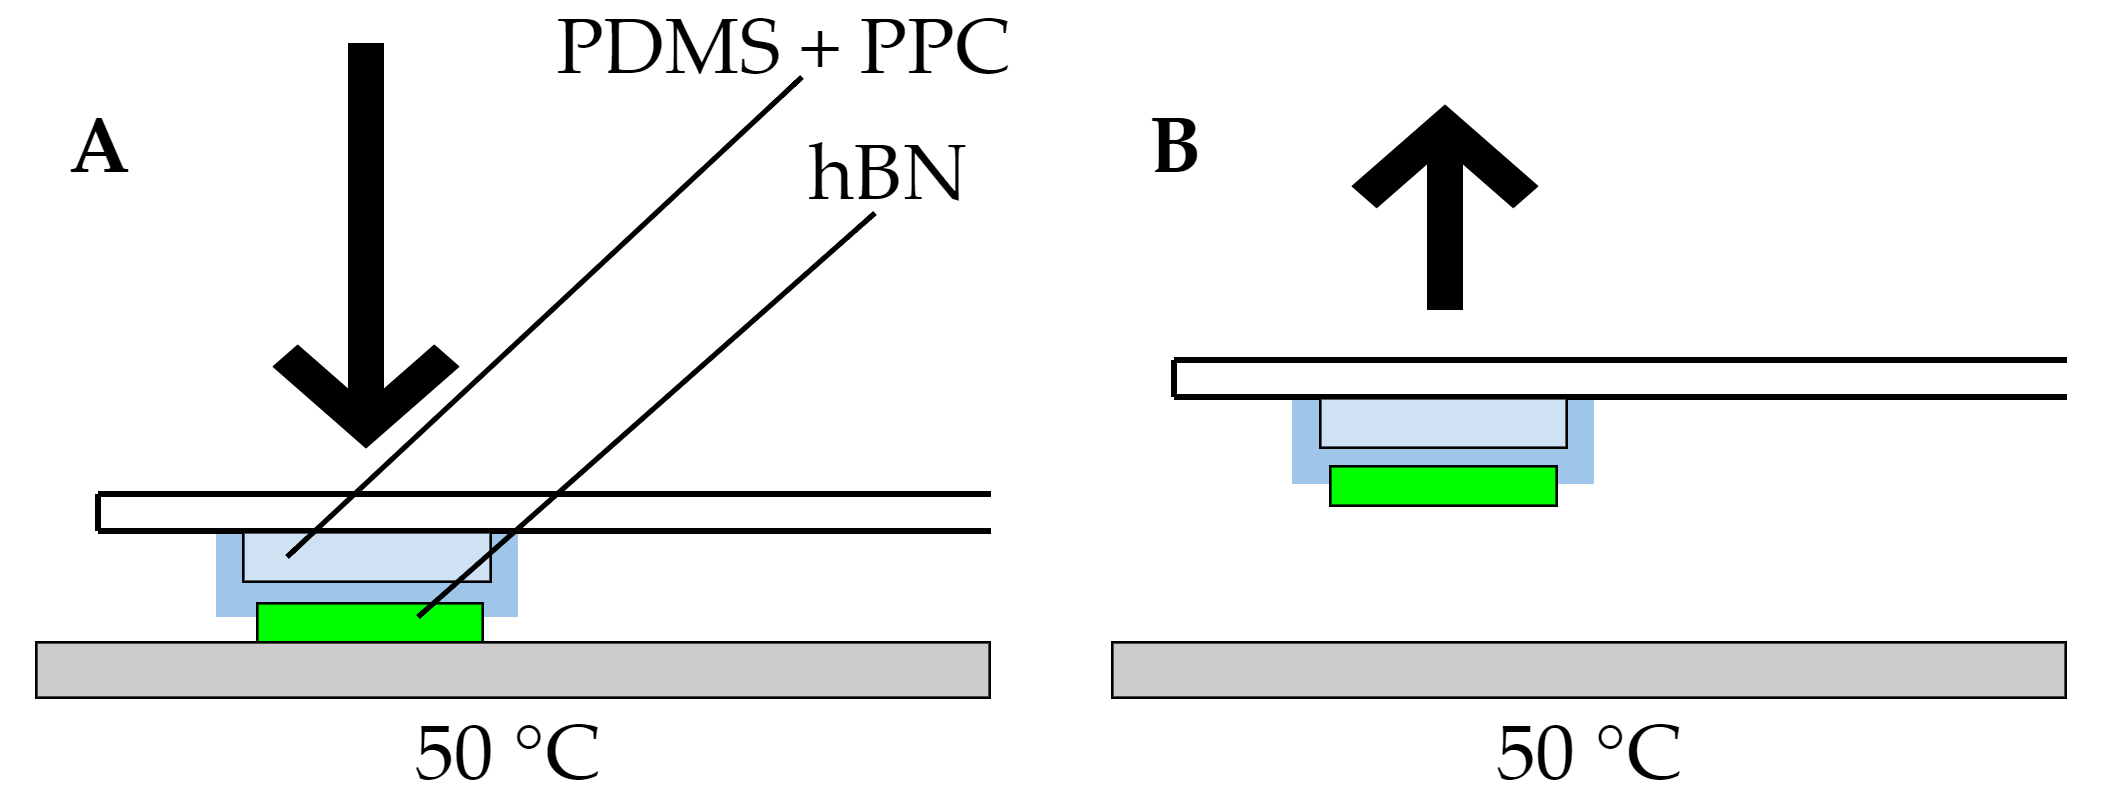
\includegraphics[width=\textwidth]{stamp_ab}

\end{subfigure}
\begin{subfigure}{0.49\textwidth}
	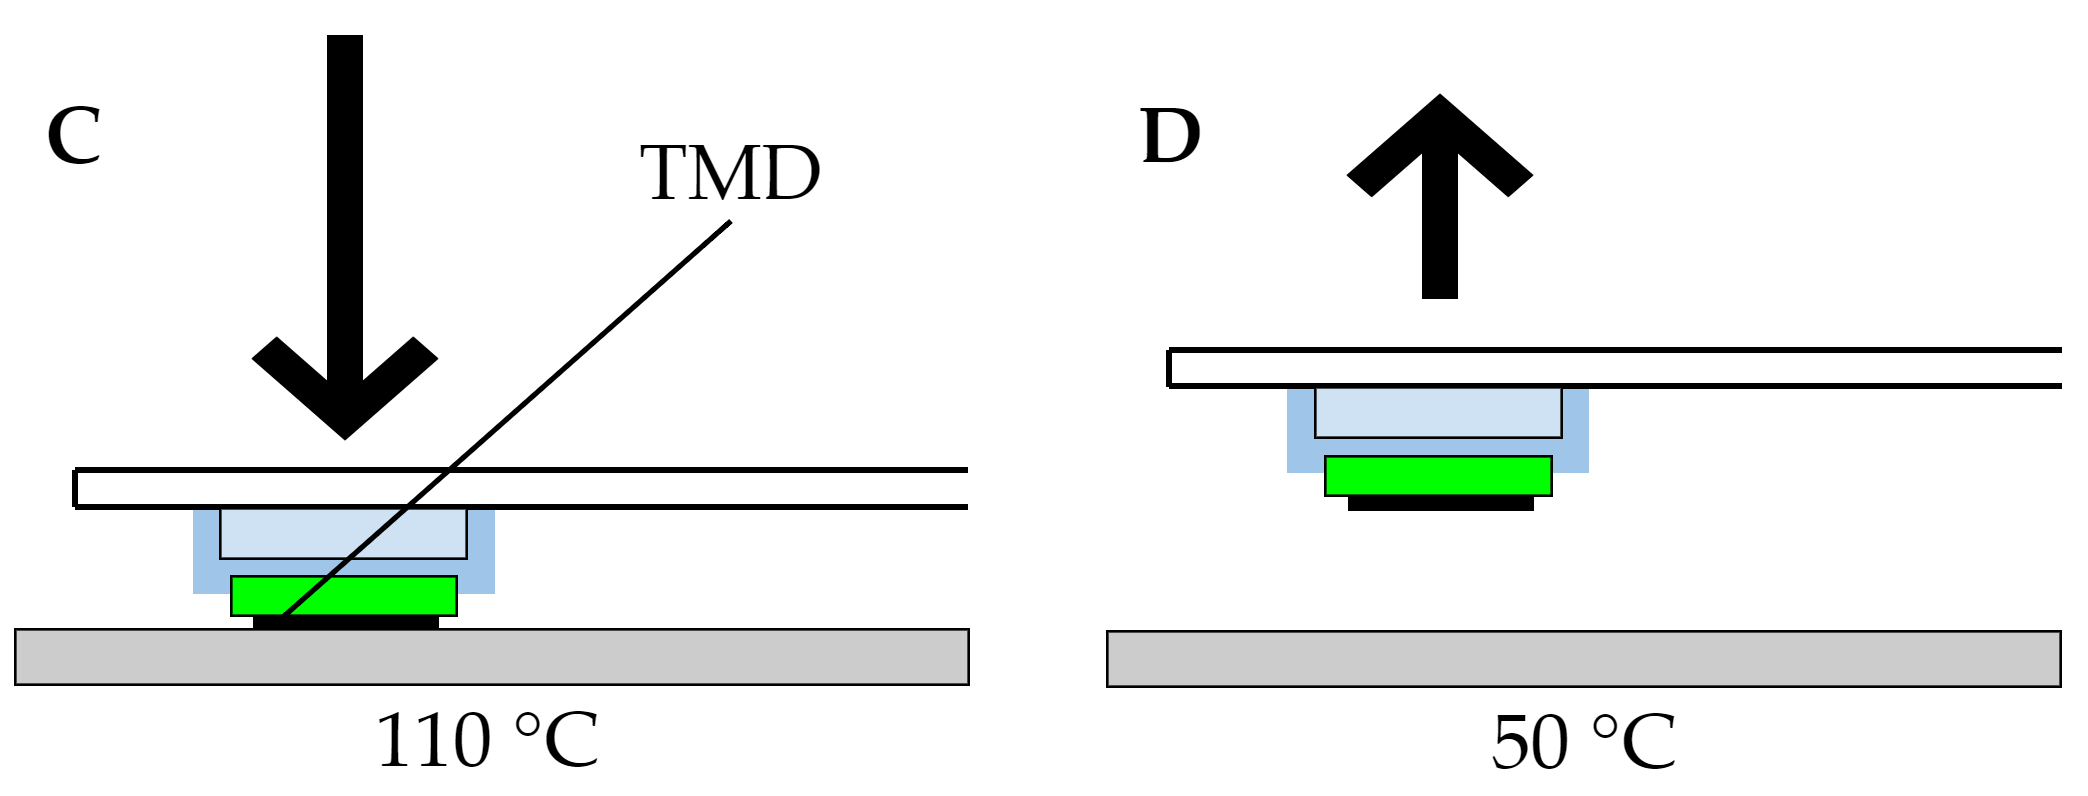
\includegraphics[width=\textwidth]{stamp_cd}
\end{subfigure}
\begin{subfigure}{0.49\textwidth}
 	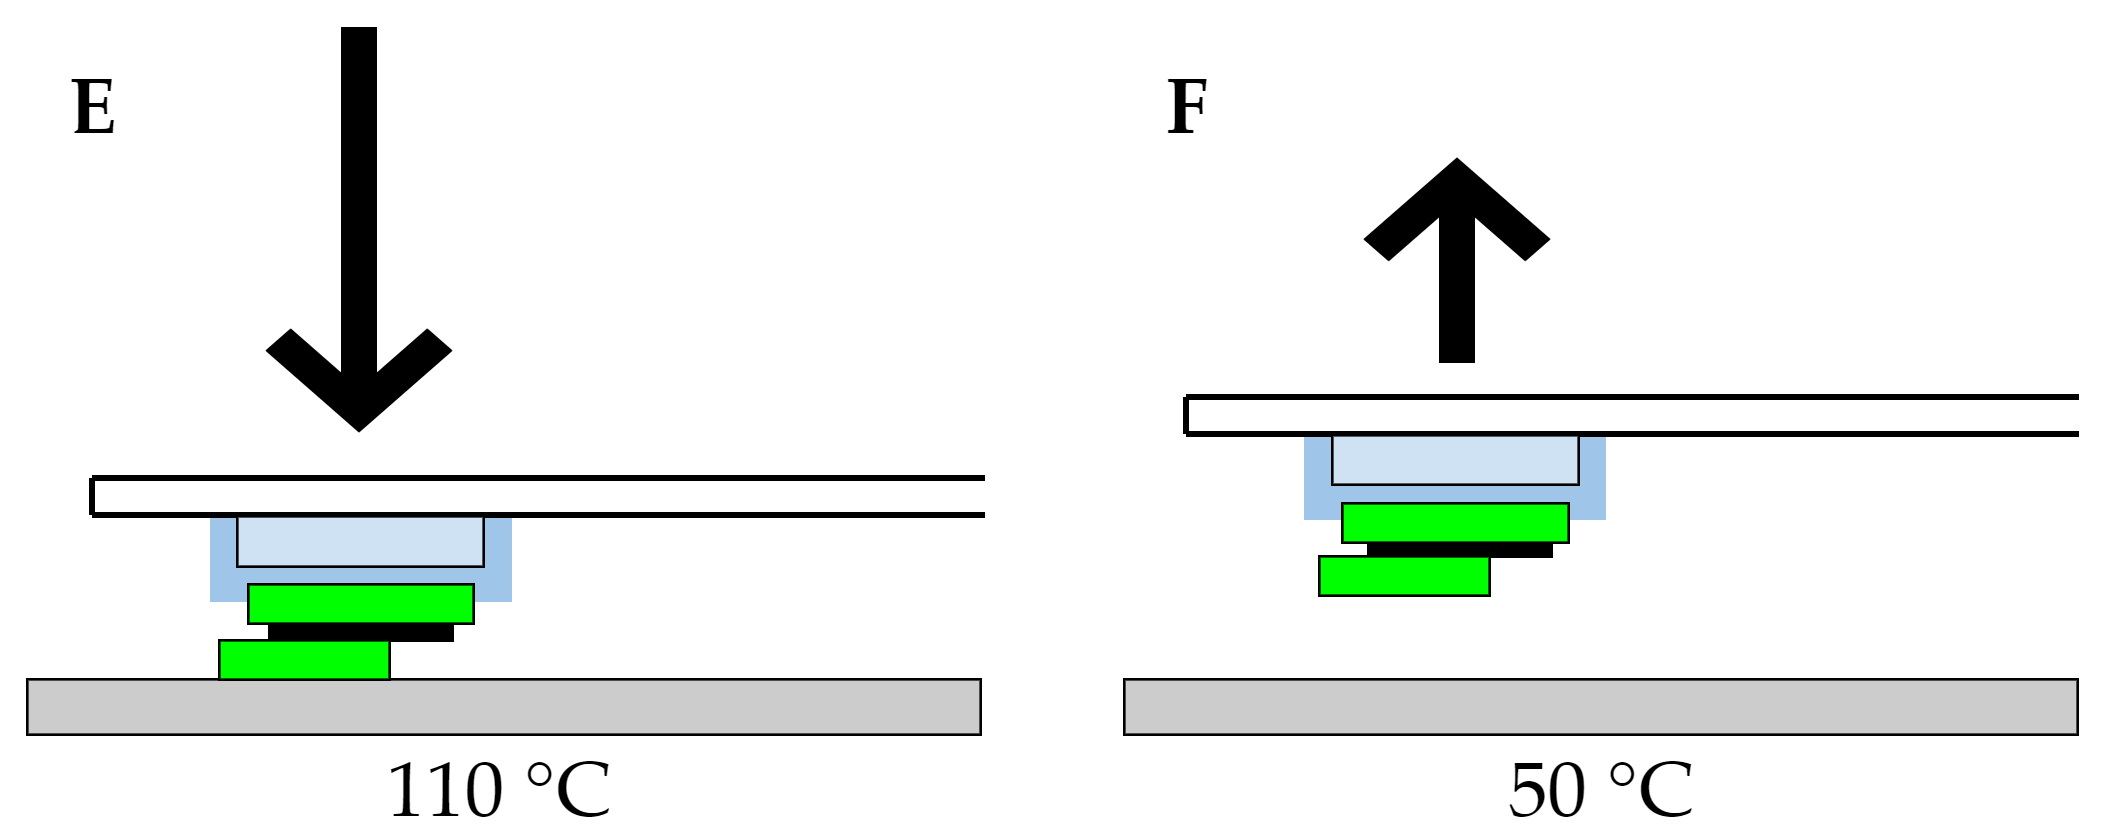
\includegraphics[width=\textwidth]{stamp_ef}

\end{subfigure}
\begin{subfigure}{0.49\textwidth}
	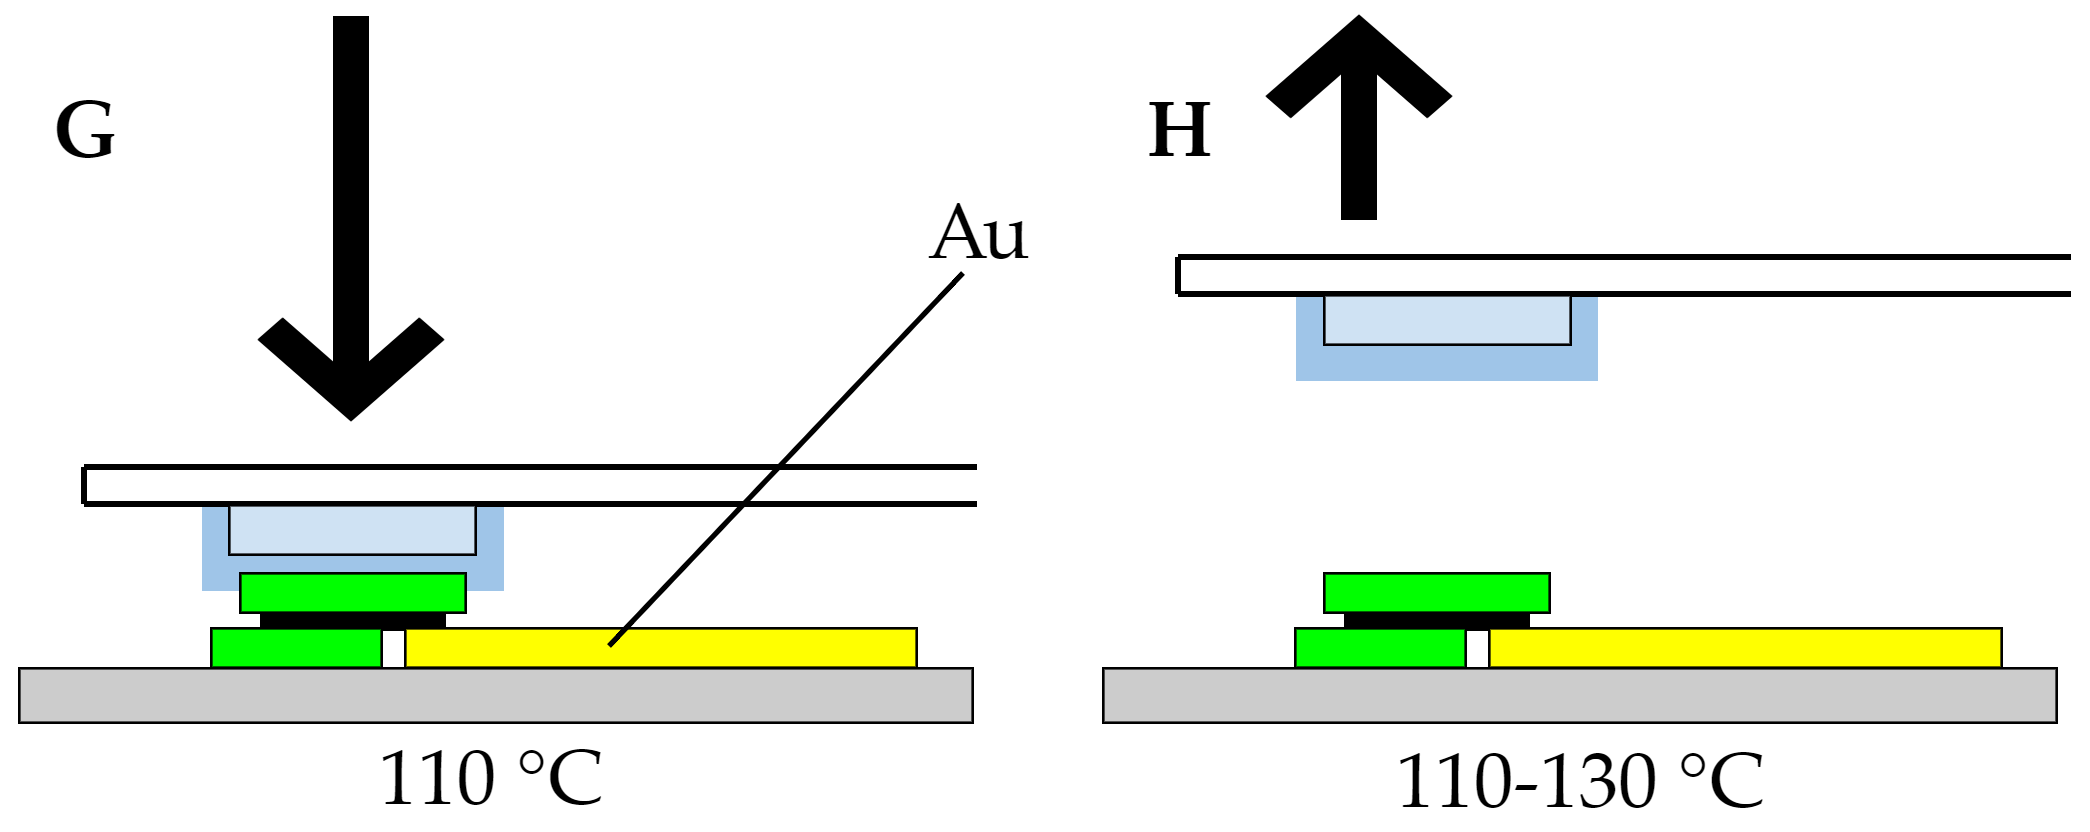
\includegraphics[width=\textwidth]{stamp_gh}
\end{subfigure}
\caption{Stamping process: "Hot pick-up and stamping" is based on strong van-der-Waals forces between \hbng and \tmds as well as the control of adhesion between \textsc{ppc} and \hbng using temperature. Flakes of \hbng are picked up from a \si/\sio substrate at 50 °C and can be dropped at a temperature around 110 °C, when the \textsc{ppc} film on the \textsc{pdms} block loses viscosity. Because thin \tmdg flakes like mono- and bilayers adhere to \hbng much better than to their substrate, the pick-up is highly reliable and arbitrarily high heterostructures can be built. To establish an electrical contact to a layer of the stack, part of it has to lay free, facing down. In this configuration the stack is simply dropped on the edge of the gold structure.}
	\label{stamping}
\end{figure}

The mechanical exfoliation method is popular also for its synergy with dry transfer methods. \textsc{Cvd}-grown \tmd-flakes are grown on suitible substrates and can be transferred to  a target substrate using a variation of wet methods, that involve powerful solvents or a combination of solvents and polymer films to lift the grown flakes off their initial substrate \cite{li_universal_2014}. The advantage of the exfoliation method in this regard is that flakes can be put on any substrate directly from the adhesive tape and do not encounter potentially damaging chemicals. This led to the invention of ``viscoelastic stamping'', where the \tmd-material is exfoliated on a substrate of viscoelastic polymer called polydimethylsiloxane (\textsc{pdms})\cite{castellanos-gomez_deterministic_2014}. This so called ``stamp'' can be brought in contact with the target substrate and peeled off carefully to drop down the flake at a desired position, opening up the possibility of producing carefully designed van-der-Waals heterostructures deterministically.

This method however can exclusively be used to drop \tmdg flakes, exfoliated directly on the stamp. This is limiting in a number of ways, since exfoliation on a polymer like \pdms\ comes with unavoidable contamination of the sensitive samples, that only gets worse with every new layer stacked on top. Attempts to develop more flexible methods to pick up \tmds and other 2\textsc{d} materials from clean substrates failed because van-der-Waals forces between the flake and a substrate like \sio could not be reliably overcome with a viscoelastic stamp. That is until \hbng was introduced as a more suitable substrate. It turns out, that van-der-Waals forces between \hbng and \tmds are high enough to remove them from \sio deterministically while a range of polymers can be used that strongly adhere to \hbng at an appropriate temperature.

This method is called ``hot pick-up and stamping''\cite{pizzocchero_hot_2016, tien_study_2016}. The stamp used in this process is a block of \textsc{pdms}, mounted on a glass slide with transparent adhesive tape. The active polymer however is polypropylene carbonate (\textsc{ppc}), that is spin-coated onto the \textsc{pdms}-block to form a thin, adhesive coating. \textsc{Ppc}, as a polar polymer sticks best to other hydrophilic substances. Therefore if the hydrophobic \textsc{pdms} is coated with \textsc{ppc} without additional treatment it can peel off, when in contact with \sio\!, especially at higher temperatures. However, the adhesion can be greatly enhanced by exposing \textsc{pdms} to oxygen plasma\cite{jung_adhesion_2016}. Before spin-coating all stamps were treated in a plasma-etching system (Gigaetch 3000) for 20 minutes, at 200 W of power.

The \tmdg and \hbn-flakes are exfoliated on a \si/\sio substrate. To raise adhesion with the flakes, these substrates are treated in oxygen plasma as well (180 s at 200 W). The primary criteria for finding the right \hbn-flakes is the flattness of its surface, so that the \tmd-flake can be encapsulated between two large terasses without cracks or steps. To allow a fast fabrication process, this flattness is only judged with help of an optical microscope. More sophisticated methods like atomic force microscopy can be used to verify the flatness more accurately. This is however much more beneficial, if the thickness of the \hbng plays an important role, for example when it is used in an optical microcavity \cite{sidler_fermi_2016}.

The goal of the hot pick-up is now to use a hot-plate to control the van-der-Waals forces between \hbn, \tmds and the substrate to ensure adhesion between the parts of the heterostructure as well as to reduce contamination with water molecules from the ambient air.

After all precursors are prepared on \si/\sio substrates, the actual pick-up and stamping process can be carried out. The fabrication setup can be seen in figure \ref{stamping-setup} and a the process in \ref{stamping}. The first step is the pick-up of the top \hbng flake. At 50°C the van-der-Waals forces between \hbng and \textsc{ppc} are already strong enough to lift the flake off the silicon substrate. Bringing flake and \textsc{ppc} in contact at a higher temperature can help as well, because this reduces the polymers viscosity. When cooling down to 40°C to 50°C afterwards, it becomes more rigid again and sticks to the \hbng more easily. In the next step the \hbng is dropped dropped on the \tmd-flake. At a higher temperature of 110°C \textsc{ppc} becomes almost fluid and peels off \hbng with ease. While the adhesion between thin \tmdg flakes and \hbng are strong enough to facilitate a pick-up also way below that temperature, heating the substrate during the drop helps to reduce the contamination with droplets of water. Since both \tmdg and \hbng flakes are prepared on clean wafers, humidity in the ambient air of the clean-room seems to be the biggest concern. Raising the temperature above the boiling point both minimizes the formation of actual droplets and also makes blisters of humid air and other contaminants at the \hbn-\tmdg interface more mobile. Dropping the stamp very slowly therefore helps to push these blisters out to the edge of the substrate\cite{pizzocchero_hot_2016}. The stack of \tmdg and \hbng can then be picked up again following the same procedure that was used for the bare \hbng flake. By repeating both steps of pick-up and drop-down an arbitrary number of layers can be added to the heterostructure. In this case it is dropped down on the bottom \hbng flake. To contact the \tmdg flake to gold part of it has to remain outside the \hbng encapsulation. This part does not necessarily have to be a monolayer but can also be any form of \tmdg, that is in contact with it so charges can be transported. The \hbng on the other hand is elastic enough so that thicker material does not affect the encapsulation of mono- or bilayer regions.

The last step is to transfer the whole stack to its final position in contact with the electrodes. This is accomplished by repeating the pick-up process once again and dropping the stack in contact with the gold structure.

Despite the strong plasma treatment of the \textsc{pdms}-stamp in some cases the \textsc{ppc} can peel off during the drop down part of the transfer due to high heat as the polymer becomes ever more liquid. In this case the sample can be carefully treated in a bath of acetone, which dissolves the polymer rapidly. The sample should stay in the bath for around one minute without any mechanical stress. Afterwards it has to be cleaned in isopropanole and blown dry with nitrogen gas. 

\subsection{Annealing}

While the hot pick-up should in theory ensure a \hbn-\tmdg interface free of contamination, especially contamination due to humidity in the ambient air can remain between the layers and seriously lower the quality of the sample. To remove this pollution, the sample can be annealed\cite{lin_graphene_2012}. During annealing, the sample is placed in an annealing oven. While maintaining a high vacuum of 10$^{-3}$ mbar, the oven heats the sample to 250°C for three hours. The vacuum ensures that any volatile materials like water vapor dissipate, while the high temperature increases the mobility of water and eventual polymer contamination on the surface. While not all dirt completely evaporates, the annealing procedure results in the formation of tiny bubbles, so that most of the interface remains clean while all dirt packs at a few avoidable places. Other recipes, that use higher or lower temperatures or longer annealing times can work just as well. Water contamination from the ambient air is still the biggest concern, so even mild temperatures should have a clear advantage over not performing the annealing-step at all. 
More aggressive recipes, that work at higher temperatures or for longer times can be more effective regarding polymer contaminations that arise from contact to the stamp. Iif the sample had to be freed of the residual \textsc{ppc} layer with acetone, contamination with polymer molecules is possible. When this exposure can be avoided however, raising the temperature has a limited advantage over milder annealing conditions, but raises also the risk of damaging the sample through temperature induced strain, that can potentially rip the \tmdg flakes. 

\section{Electrical characterization}

To assess the quality of the the gate structure, its breakdown voltage has to be determined. This is the voltage between top gate and back gate, at which the leakage current starts to rise exponentially by forming conducting channels through the dielectric, that are self-sustaining and lift the conductance permanently\cite{klein_maximum_1966}. This breakdown voltage is complicated to predict, as it is a nonlinear effect mainly caused by faults in the \sio layer. Thus it does not only depend on the thickness of the dielectric but also on the area of the top gate, because the statistical chance of encounterin a fault in the material and a conducting channel forming is higher the more area of the sample is covered with conducting material. Additionally the rather violent ohmic contacting of the backgate can also damage the dielectric and lower the breakdown voltage. Therefore each sample has to be classified before being used to tune the charge density in optical spectroscopy. The dielectric in samples used throughout this thesis had a thickness of 50 nm or 90 nm, corresponding to a predicted breakdown voltage of 47.5 V or 85.5 V respectively. To verify these values, the leakage currents have to be monitored while ramping up the voltage. Before breakdown these currents are of the order of 100 pA to 1 nA and can be measured using a lock-in amplifier. A diagram of the circuitry is drawn in figure \ref{cv}. A constant voltage across the desired range of operation ({\small$\pm $}30V) is added to a small \textsc{ac}-voltage of small amplitude ($U_0 = $ 10 mV$_{pp}$, $f = $ 77.1 Hz). The amplifyer can monitor the real and imaginary part of the current. The real part is the resistive current, or leakage, that flows through the samples dielectric. The imaginary part is proportional to the capacity. By first performing the experiment with a gauge capacitance, the capacity of the sample can be measured with high precision. For the purpose of characterizing the dielectric however, the resistive current is the more interesting quantity. To find the breakdown voltage the \textsc{dc}-voltage is ramped until the leakage rises exponentially. At this voltage, the resistive current is still usually still below a few nA---small enough to not inflict permanent damage to the dielectric and marks a safe range of positive and negative voltages the device can be operated on during the experiment.

\begin{figure}
	\centering
	\resizebox{!}{150pt}{%
	\begin{tikzpicture}[scale=0.62, every node/.append style={transform shape}]
	\begin{circuitikz}
		\draw (0,0) to[short] (0,0);
		\draw 
		(0,6) to[short, o-] (0,3)
		(0,3) to[R, l=$10k\Omega$,-*] (2,3) 
		(2,1) to[C, l=$2.2 \mu$F] (2,3) 
		(2,1) node[ground]{}
		(2,3) to[R, l=$100k\Omega$] (4,3) -- (7,3)
		(5,3) to[C, l=$0.68\mu$F,*-] (5,5)
		(5,5) to[short, -o] (5,6)
		(7,3) to[short, -o] (7,2)
		(8,2) to[short, o-] (8,3) -- (10,3)
		(7,6) to[short, o-] (7,5)
			 to[short] (8,5)
		(8,5) to[short, -o] (8,6)
		(10,3) to[short, -o] (10,6)
		;
		\node at (7.5,4.7) {$77.1$Hz};
		\node at (6.15,2) {Topgate};
		\node at (9,2) {Backgate};
		\draw (-0.4,5.5) -- (-0.4,7) -- (2.2,7) -- (2.2,5.5) -- (-0.4,5.5);
		\draw (4.6,5.5) -- (4.6,7) -- (7.4,7) -- (7.4,5.5) -- (4.6,5.5);
		\draw (7.6,5.5) -- (7.6,7) -- (10.4,7) -- (10.4,5.5) -- (7.6,5.5);
		\node[align=left] at (1,6.5) {DC-Voltage\\source};
		\node[align=left] at (6.1,6.5) {AC-function\\generator};
		\node[align=left] at (8.9,6.5) {Lock-in\\amplifier};
	\end{circuitikz}

	\end{tikzpicture}
	}
	\caption{Diagram for the \textsc{cv}-measurement. Using a lock-in amplifier and a small \textsc{ac} voltage even very small resistive currents leaking through the samples dielectric can be measured. This way, the maximum \textsc{dc} voltage at the gate can be obtained, by ramping a \textsc{dc} voltage source until the resistive current starts to rise exponentially.}\label{cv}
\end{figure}